\documentclass[onecolumn, compsoc,12pt]{IEEEtran}
\usepackage{enumitem}
\usepackage{floatrow}
\floatsetup[table]{capposition=top}
\usepackage{etex}
\usepackage{amssymb,amsfonts,amsmath,amsthm}
\usepackage{graphicx}
 \usepackage[usenames,x11names, dvipsnames, svgnames]{xcolor}
\usepackage{amsmath,amssymb}
\usepackage{dsfont}
\usepackage{amsfonts}
\usepackage{mathrsfs}
\usepackage{hyperref}
\hypersetup{
    colorlinks=true,
    linkcolor=black,
    citecolor=MediumBlue,
    filecolor=black,
    urlcolor=DodgerBlue4,
    breaklinks=false,
%linkbordercolor=red,% hyperlink borders will be red
  %pdfborderstyle={/S/U/W 1}% border style will be underline of width 1pt
}
\usepackage{array}
%\usepackage{multirow}    
%\usepackage[T1,euler-digits]{eulervm}
%\usepackage{times}
%\usepackage{pxfonts}
\usepackage{tikz}
\usepackage{pgfplots}
\usetikzlibrary{shapes,calc,shadows,fadings,arrows,decorations.pathreplacing,automata,positioning}
\usetikzlibrary{external}
\usetikzlibrary{decorations.text}
\usepgfplotslibrary{colorbrewer} 
\tikzexternalize[prefix=./Figures/External/]% activate externalization!
\tikzexternaldisable
%\addtolength{\voffset}{.1in}  
\usepackage{geometry}
\geometry{a4paper, left=.95in,right=.95in,top=.95in,bottom=0.95in}

%\addtolength{\textwidth}{-.1in}    
%\addtolength{\hoffset}{.05in}    
%\addtolength{\textheight}{.1in}    
%\addtolength{\footskip}{0in}    
\usepackage{rotating}
 \definecolor{nodecol}{RGB}{240,240,220}
 \definecolor{nodeedge}{RGB}{240,240,225}
  \definecolor{edgecol}{RGB}{130,130,130}
    \tikzset{%
fshadow/.style={      preaction={
         fill=black,opacity=.3,
         path fading=circle with fuzzy edge 20 percent,
         transform canvas={xshift=1mm,yshift=-1mm}
       }} 
}
\usetikzlibrary{pgfplots.dateplot}
 \usetikzlibrary{patterns}
\usetikzlibrary{decorations.markings}
\usepackage{fancyhdr}
\renewcommand{\headrulewidth}{0pt}
\usepackage{mathtools}
\usepackage{datetime}
\usepackage{comment}
%% ## Equation Space Control---------------------------
\def\EQSP{4pt}
\newcommand{\mltlne}[2][\EQSP]{\begingroup\setlength\abovedisplayskip{#1}\setlength\belowdisplayskip{#1}\begin{equation}\begin{multlined} #2 \end{multlined}\end{equation}\endgroup}
\newcommand{\cgather}[2][\EQSP]{\begingroup\setlength\abovedisplayskip{#1}\setlength\belowdisplayskip{#1}\begin{gather} #2 \end{gather}\endgroup}
\newcommand{\cgathers}[2][\EQSP]{\begingroup\setlength\abovedisplayskip{#1}\setlength\belowdisplayskip{#1}\begin{gather*} #2 \end{gather*}\endgroup}
\newcommand{\calign}[2][\EQSP]{\begingroup\setlength\abovedisplayskip{#1}\setlength\belowdisplayskip{#1}\begin{align} #2 \end{align}\endgroup}
\newcommand{\caligns}[2][\EQSP]{\begingroup\setlength\abovedisplayskip{#1}\setlength\belowdisplayskip{#1}\begin{align*} #2 \end{align*}\endgroup}
\newcommand{\mnp}[2]{\begin{minipage}{#1}#2\end{minipage}} 
%% COLOR DEFS------------------------------------------
\newtheorem{thm}{Theorem}
\newtheorem{cor}{Corollary}
\newtheorem{lem}{Lemma}
\newtheorem{prop}{Proposition}
\newtheorem{defn}{Definition}
\newtheorem{example}{Example}
\newtheorem{rem}{Remark}
\newtheorem{notn}{Notation}
%%------------PROOF INCLUSION -----------------
\def\NOPROOF{Proof omitted.}
\newif\ifproof
\prooffalse % or \draftfalse
\newcommand{\Proof}[1]{
\ifproof
\begin{IEEEproof}
#1\end{IEEEproof}
\else
\NOPROOF
\fi
 }
%%------------ -----------------
\newcommand{\DETAILS}[1]{#1}
%%------------ -----------------
% color commands------------------------
\newcommand{\etal}{\textit{et} \mspace{3mu} \textit{al.}}
% \renewcommand{\algorithmiccomment}[1]{$/** $ #1 $ **/$}
\newcommand{\vect}[1]{\textbf{\textit{#1}}}
\newcommand{\figfont}{\fontsize{8}{8}\selectfont\strut}
\newcommand{\hlt}{ \bf \sffamily \itshape\color[rgb]{.1,.2,.45}}
\newcommand{\pitilde}{\widetilde{\pi}}
\newcommand{\Pitilde}{\widetilde{\Pi}}
\newcommand{\bvec}{\vartheta}
\newcommand{\algo}{\textrm{\bf\texttt{GenESeSS}}\xspace}
\newcommand{\xalgo}{\textrm{\bf\texttt{xGenESeSS}}\xspace}
\newcommand{\FNTST}{\bf }
\newcommand{\FNTED}{\color{darkgray} \scriptsize $\phantom{.}$}
\renewcommand{\baselinestretch}{.93}
\newcommand{\sync}{\otimes}
\newcommand{\psync}{\hspace{3pt}\overrightarrow{\hspace{-3pt}\sync}}
%\newcommand{\psync}{\raisebox{-4pt}{\begin{tikzpicture}\node[anchor=south] (A) {$\sync$};
%\draw [->,>=stealth] ([yshift=-2pt, xshift=2pt]A.north west) -- ([yshift=-2pt]A.north east); %\end{tikzpicture}}}
\newcommand{\base}[1]{\llbracket #1 \rrbracket}
\newcommand{\nst}{\textrm{\sffamily\textsc{Numstates}}}
\newcommand{\HA}{\boldsymbol{\mathds{H}}}
\newcommand{\eqp}{ \vartheta }
\newcommand{\entropy}[1]{\boldsymbol{h}\left ( #1 \right )}
\newcommand{\norm}[1]{\left\lVert #1 \right\rVert}%
\newcommand{\abs}[1]{\left\lvert #1 \right\rvert}%
\newcommand{\absB}[1]{\big\lvert #1 \big\rvert}%
% #############################################################
% #############################################################
% PREAMBLE ####################################################
% #############################################################
% #############################################################
% \usepackage{pnastwoF}
\DeclareMathOperator*{\argmax}{argmax}
\newcommand{\ND}{ \mathcal{N}  }
\usepackage[linesnumbered,ruled,vlined,noend]{algorithm2e}
\newcommand{\captionN}[1]{\caption{\color{darkgray} \sffamily \fontsize{8}{10}\selectfont #1  }}
\newcommand{\btl}{\ \textbf{\small\sffamily bits/letter}}
\usepackage{txfonts}
\usepackage{times}
%\usepackage{ccfonts}
%%% save defaults
%\renewcommand{\rmdefault}{phv} % Arial
%\renewcommand{\sfdefault}{phv} % Arial
\edef\keptrmdefault{\rmdefault}
\edef\keptsfdefault{\sfdefault}
\edef\keptttdefault{\ttdefault}

%\usepackage{kerkis}
\usepackage[OT1]{fontenc}
\usepackage{concmath}
%\usepackage[T1]{eulervm}
%\usepackage[OT1]{fontenc}
%%% restore defaults
\edef\rmdefault{\keptrmdefault}
\edef\sfdefault{\keptsfdefault}
\edef\ttdefault{\keptttdefault}
\tikzexternalenable
% ##########################################################
\tikzfading[name=fade out,
            inner color=transparent!0,
            outer color=transparent!100]
%###################################
\newcommand{\xtitaut}[2]{
\noindent\mnp{\textwidth}{
\mnp{\textwidth}{\raggedright\Huge \bf \sffamily #1}

\vskip 1em

{\bf \sffamily #2}
}
\vskip 2em
}
%###################################
%###################################
\tikzset{wiggle/.style={decorate, decoration={random steps, amplitude=10pt}}}
\usetikzlibrary{decorations.pathmorphing}
\pgfdeclaredecoration{Snake}{initial}
{
  \state{initial}[switch if less than=+.625\pgfdecorationsegmentlength to final,
                  width=+.3125\pgfdecorationsegmentlength,
                  next state=down]{
    \pgfpathmoveto{\pgfqpoint{0pt}{\pgfdecorationsegmentamplitude}}
  }
  \state{down}[switch if less than=+.8125\pgfdecorationsegmentlength to end down,
               width=+.5\pgfdecorationsegmentlength,
               next state=up]{
    \pgfpathcosine{\pgfqpoint{.25\pgfdecorationsegmentlength}{-1\pgfdecorationsegmentamplitude}}
    \pgfpathsine{\pgfqpoint{.25\pgfdecorationsegmentlength}{-1\pgfdecorationsegmentamplitude}}
  }
  \state{up}[switch if less than=+.8125\pgfdecorationsegmentlength to end up,
             width=+.5\pgfdecorationsegmentlength,
             next state=down]{
    \pgfpathcosine{\pgfqpoint{.25\pgfdecorationsegmentlength}{\pgfdecorationsegmentamplitude}}
    \pgfpathsine{\pgfqpoint{.25\pgfdecorationsegmentlength}{\pgfdecorationsegmentamplitude}}
  }
  \state{end down}[width=+.3125\pgfdecorationsegmentlength,
                   next state=final]{
     \pgfpathcosine{\pgfqpoint{.15625\pgfdecorationsegmentlength}{-.5\pgfdecorationsegmentamplitude}}
     \pgfpathsine{\pgfqpoint{.15625\pgfdecorationsegmentlength}{-.5\pgfdecorationsegmentamplitude}}
  }
  \state{end up}[width=+.3125\pgfdecorationsegmentlength,
                 next state=final]{
     \pgfpathcosine{\pgfqpoint{.15625\pgfdecorationsegmentlength}{.5\pgfdecorationsegmentamplitude}}
     \pgfpathsine{\pgfqpoint{.15625\pgfdecorationsegmentlength}{.5\pgfdecorationsegmentamplitude}}
  }
  \state{final}{\pgfpathlineto{\pgfpointdecoratedpathlast}}
}
%###################################
%###################################
\newcolumntype{L}[1]{>{\rule{0pt}{2ex}\raggedright\let\newline\\\arraybackslash\hspace{0pt}}m{#1}}
\newcolumntype{C}[1]{>{\rule{0pt}{2ex}\centering\let\newline\\\arraybackslash\hspace{0pt}}m{#1}}
\newcolumntype{R}[1]{>{\rule{0pt}{2ex}\raggedleft\let\newline\\\arraybackslash\hspace{0pt}}m{#1}}




\newcommand{\drhh}[8]{
\begin{axis}[semithick,
font=\bf \sffamily \fontsize{7}{7}\selectfont,
name=H2,
at=(#4), anchor=#5,
xshift=.3in,
yshift=-.3in,
width=\WDT, 
height=\HGT, 
title={{\LARGE G } ROC area distribution (Out-of-sample)}, 
title style={align=right, },legend cell align=left,
legend style={ xshift=3.5in, yshift=-.6in, draw=white, fill= gray, fill opacity=0.2, 
text opacity=1,},
axis line style={black!80, opacity=0,   thick,,ultra thin, rounded corners=0pt},
axis on top=false, 
xlabel={ROC area},
ylabel={probability},
ylabel style={yshift=-.25in},
xlabel style={yshift=.1in},
grid style={dashed, gray!50},
%grid,
axis background/.style={top color=gray!1,bottom color=gray!2},
enlargelimits=false, 
scale only axis=true,
ymin=0,
%xmin=.7,xmax=1.0,
ylabel style={yshift=.05in},
major tick length=0pt,yticklabel style={/pgf/number format/fixed,/pgf/number format/precision=2},xticklabel style={/pgf/number format/fixed,/pgf/number format/precision=2},
#7,
 ]
\addplot [
    fill=#8,
    thick,
    draw=white,
    opacity=1,
    hist={density,bins=10},
] table [y index=#3] {#1};
% \addlegendentry{$\Delta$ ROC};
\addplot [very thick, Red2,, opacity=.95] gnuplot [raw gnuplot] {plot '#1' u #2:(1./#6.) smooth kdensity};
%
%\draw[thin,black ] (axis cs:.89291,\pgfkeysvalueof{/pgfplots/ymin}) -- (axis cs:.89291,\pgfkeysvalueof{/pgfplots/ymax}) node [midway,right, pos=0.2] {89.3\%};
% \addlegendentry{kde};
\end{axis}
}


\newcommand{\erhh}[6]{
  \begin{axis}[semithick,
font=\bf \sffamily \fontsize{7}{7}\selectfont,
name=H2,
at=(#3), anchor=#4,
xshift=.3in,
yshift=-.3in,
width=\WDT, 
height=\HGT, 
title style={align=center, },legend cell align=left,
legend style={ xshift=3.5in, yshift=-.6in, draw=white, fill= gray, fill opacity=0.2, 
text opacity=1,},
axis line style={black!80, opacity=0,   thick,,ultra thin, rounded corners=0pt},
axis on top=false, 
xlabel={ROC area},
ylabel={probability},
ylabel style={yshift=-.25in},
xlabel style={yshift=.1in},
grid style={dashed, gray!50},
%grid,
axis background/.style={top color=gray!1,bottom color=gray!2},
enlargelimits=false, 
scale only axis=true,
%ymin=0, 
%xmin=.7,xmax=1.0,
ylabel style={yshift=.05in},
major tick length=0pt,yticklabel style={/pgf/number format/fixed,/pgf/number format/precision=2},xticklabel style={/pgf/number format/fixed,/pgf/number format/precision=2},
#5,
 ]
    \addplot[semithick, #6]
    table[x expr=(\coordindex+1),y expr=(\thisrowno{#2})] {#1};
    % \addlegendentry{Cullman, Alabama};
  \end{axis}
}
%################################################
%################################################
%################################################
%################################################
\def\DISCLOSURE#1{\def\disclosure{#1}}
\DISCLOSURE{\raisebox{15pt}{$\phantom{XxxX}$This sheet contains proprietary information 
 not to be released to third parties except for the explicit purpose of evaluation.}
}
\newcommand{\acomment}[1]{\vskip 1em {\color{gray} #1} \vskip 1em}


% ####################################
\newcommand{\set}[1]{\left\{ #1 \right\}}
\newcommand{\paren}[1]{\left( #1 \right)}
\newcommand{\bracket}[1]{\left[ #1 \right]}
% \newcommand{\norm}[1]{\left\Vert #1 \right\Vert}
\newcommand{\nrm}[1]{\left\llbracket{#1}\right\rrbracket}
\newcommand{\parenBar}[2]{\paren{#1\,{\left\Vert\,#2\right.}}}
\newcommand{\parenBarl}[2]{\paren{\left.#1\,\right\Vert\,#2}}
\newcommand{\ie}{$i.e.$\xspace}
\newcommand{\addcitation}{\textcolor{black!50!red}{\textbf{ADD CITATION}}}
\newcommand{\subtochange}[1]{{\color{black!50!green}{#1}}}
\newcommand{\tobecompleted}{{\color{black!50!red}TO BE COMPLETED.}}


\newcommand{\pIn}{\mathscr{P}_{\textrm{in}}}
\newcommand{\pOut}{\mathscr{P}_{\textrm{out}}}
\newcommand{\aIn}[1][\Sigma]{#1_{\textrm{in}}}
\newcommand{\aOut}[1][\Sigma]{#1_{\textrm{out}}}
\newcommand{\xin}[1]{#1_{\textrm{in}}}
\newcommand{\xout}[1]{#1_{\textrm{out}}}

\newcommand{\R}{\mathbb{R}} % Set of real numbers
\newcommand{\F}[1][]{\mathcal{F}_{#1}}
\newcommand{\SR}{\mathcal{S}} % Semiring of sets
\newcommand{\RR}{\mathcal{R}} % Ring of sets
\newcommand{\N}{\mathbb{N}} % Set of natural numbers (0 included)


\newcommand{\Pp}[1][n]{\mathscr{P}^+_{#1}}
\renewcommand{\entropy}[1]{\boldsymbol{h}\left ( #1 \right )}



\makeatletter
\pgfdeclarepatternformonly[\hatchdistance,\hatchthickness]{flexible hatch}
{\pgfqpoint{0pt}{0pt}}
{\pgfqpoint{\hatchdistance}{\hatchdistance}}
{\pgfpoint{\hatchdistance-1pt}{\hatchdistance-1pt}}%
{
  \pgfsetcolor{\tikz@pattern@color}
  \pgfsetlinewidth{\hatchthickness}
  \pgfpathmoveto{\pgfqpoint{0pt}{0pt}}
  \pgfpathlineto{\pgfqpoint{\hatchdistance}{\hatchdistance}}
  \pgfusepath{stroke}
}
\makeatother

\pgfdeclarepatternformonly{north east lines wide}%
{\pgfqpoint{-1pt}{-1pt}}%
{\pgfqpoint{10pt}{10pt}}%
{\pgfqpoint{9pt}{9pt}}%
{
  \pgfsetlinewidth{0.7pt}
  \pgfpathmoveto{\pgfqpoint{0pt}{0pt}}
  \pgfpathlineto{\pgfqpoint{9.1pt}{9.1pt}}
  \pgfusepath{stroke}
}

\pgfdeclarepatternformonly{north west lines wide}%
{\pgfqpoint{-1pt}{-1pt}}%
{\pgfqpoint{10pt}{10pt}}%
{\pgfqpoint{9pt}{9pt}}%
{
  \pgfsetlinewidth{0.7pt}
  \pgfpathmoveto{\pgfqpoint{0pt}{9pt}}
  \pgfpathlineto{\pgfqpoint{9.1pt}{-0.1pt}}
  \pgfusepath{stroke}
}
\makeatletter

\pgfdeclarepatternformonly[\hatchdistance,\hatchthickness]{flexible hatchB}
{\pgfqpoint{0pt}{\hatchdistance}}
{\pgfqpoint{\hatchdistance}{0pt}}
{\pgfpoint{1pt}{\hatchdistance-1pt}}%
{
  \pgfsetcolor{\tikz@pattern@color}
  \pgfsetlinewidth{\hatchthickness}
  \pgfpathmoveto{\pgfqpoint{0pt}{\hatchdistance}}
  \pgfpathlineto{\pgfqpoint{\hatchdistance}{0pt}}
  \pgfusepath{stroke}
}    \makeatother


\def\TPR{\textrm{TPR}\xspace}
\def\TNR{\textrm{TNR}\xspace}
\def\FPR{\textrm{FPR}\xspace}
\def\PPV{\textrm{PPV}\xspace}

\usetikzlibrary{arrows.meta}
\usetikzlibrary{decorations.pathreplacing,shapes.misc}
\usepgfplotslibrary{fillbetween}
%usepackage{tikz-network}
\usetikzlibrary{shapes.geometric}
\usetikzlibrary{math}
\usepgfplotslibrary{colorbrewer} 

\usepackage{textcomp}
\usepackage{colortbl}
\usepackage{array}
\usepackage{courier} 
\usepackage{wrapfig}
\usepackage{pifont}
\usetikzlibrary{chains,backgrounds}
\usetikzlibrary{intersections}
\usetikzlibrary{pgfplots.groupplots}
\usepgfplotslibrary{fillbetween} 
\usetikzlibrary{arrows.meta}
\usepackage{pgfplotstable}
%\usepackage{cite}
\usepackage[super,compress,sort,comma]{natbib}
%\usepackage{natbib}
\usepackage{setspace}
\usetikzlibrary{math}
\usetikzlibrary{matrix}
\usepackage{xstring}
\usepackage{xspace}
\usepackage{flushend}
\makeatletter
\renewcommand\section{\@startsection {section}{1}{\z@}%
  {-2ex \@plus -1ex \@minus -.2ex}%
  {1ex \@plus.1ex}%
  {\Large\bfseries\scshape}}
\renewcommand\subsection{\@startsection {section}{1}{\z@}%
  {-2ex \@plus -.25ex \@minus -.2ex}%
  {0.1ex \@plus.0ex}%
  {\fontsize{11}{10}\selectfont\bfseries\sffamily\color{black}}}
\renewcommand\subsubsection{\@startsection {section}{1}{\z@}%
  {0ex \@plus -.5ex \@minus -.2ex}%
  {0.0ex \@plus.5ex}%
  {\fontsize{9}{9}\selectfont\bfseries\itshape\sffamily\color{darkgray}}}
\renewcommand\paragraph{\@startsection {section}{1}{\z@}%
  {-.2ex \@plus -.5ex \@minus -.2ex}%
  {0.0ex \@plus.5ex}%
  {\fontsize{9}{9}\selectfont\itshape\sffamily\color{darkgray}}}
       
 
\makeatother
\makeatletter
\pgfdeclareradialshading[tikz@ball]{ball}{\pgfqpoint{-10bp}{10bp}}{%
  color(0bp)=(tikz@ball!30!white);
  color(9bp)=(tikz@ball!75!white);
  color(18bp)=(tikz@ball!90!black);
  color(25bp)=(tikz@ball!70!black);
  color(50bp)=(black)}
\makeatother
%\newcommand{\tball}[1][CadetBlue4]{${\color{#1}\Large\boldsymbol{\blacksquare}}$}
\renewcommand{\baselinestretch}{1}
%\renewcommand{\captionN}[1]{\caption{\color{CadetBlue4!50!black} \sffamily \fontsize{9}{10}\selectfont #1  }}
\tikzexternaldisable 
\parskip=2pt
\parindent=0pt
%\newcommand{\Mark}[1]{\textsuperscript{#1}}
\pagestyle{fancy}

\newcounter{Dcounter}
\setcounter{Dcounter}{1}
\newif\ifdraftQ
\newcommand{\DQS}[1]{\ifdraftQ
{\marginpar{\tikzexternaldisable \tikz{\node[rounded corners=5pt,draw=none,thick,fill=black!10,font=\sffamily\fontsize{7}{8}\selectfont] {\mnp{.45in} {\color{Red3}\raggedright  \#\theDcounter.~#1}}; }}}\stepcounter{Dcounter}\xspace
\fi}

\newcommand{\qn}[1][i]{\Phi_{#1}}
\newcommand{\D}[1][i]{\mathscr{D}\left ( {\Sigma_#1} \right ) }
\newcommand{\Dx}{\mathscr{D}}
\def\J{\mathds{J}}
\def\M{\omega}
\def\N{\mathds{N}}
\newcommand{\cp}[1][P]{\langle #1 \rangle}
\newcommand{\mem}[1]{\M_{#1}}


\makeatletter
\newcommand\transformxdimension[1]{
    \pgfmathparse{((#1/\pgfplots@x@veclength)+\pgfplots@data@scale@trafo@SHIFT@x)/10^\pgfplots@data@scale@trafo@EXPONENT@x}
}
\newcommand\transformydimension[1]{
    \pgfmathparse{((#1/\pgfplots@y@veclength)+\pgfplots@data@scale@trafo@SHIFT@y)/10^\pgfplots@data@scale@trafo@EXPONENT@y}
}
\makeatother

\parskip=6pt
\parindent=0pt


\pgfplotsset{
    discard if/.style 2 args={
        x filter/.code={
            \edef\tempa{\thisrow{#1}}
            \edef\tempb{#2}
            \ifx\tempa\tempb
                \def\pgfmathresult{inf}
            \fi
        }
    },
    discard if not/.style 2 args={
        x filter/.code={
            \edef\tempa{\thisrow{#1}}
            \edef\tempb{#2}
            \ifx\tempa\tempb
            \else
                \def\pgfmathresult{inf}
            \fi
        }
    }
  }

  
\makeatletter
\newcommand{\limitpages}[1]{
    \gdef\maxpages{#1}%
    \ifx\latex@outputpage\@undefined\relax%
        \global\let\latex@outputpage\@outputpage%
    \fi%
    \gdef\@outputpage{%
        \ifnum\value{page}>\maxpages\relax%
            % Do not output the page
        \else%
            \latex@outputpage%
        \fi%
    }%
}
\makeatother
 
%\usepackage{cite}
\usepackage{textcomp}
\usepackage{colortbl}
\usepackage{subfigure}
\usepackage{array}
\usepackage{courier}
\usepackage{setspace} 
\usepackage{wrapfig} 
\usepackage{calligra}
\usepackage{ulem}
\usepackage{multirow}
\renewcommand{\IEEEbibitemsep}{20pt plus 2pt}
\makeatletter
\IEEEtriggercmd{\reset@font\normalfont\fontsize{11}{14}\selectfont}
\makeatother
\IEEEtriggeratref{1}
\newlength{\bibitemsep}\setlength{\bibitemsep}{.2\baselineskip plus .05\baselineskip minus .05\baselineskip}
\newlength{\bibparskip}\setlength{\bibparskip}{0pt}
\let\oldthebibliography\thebibliography
\renewcommand\thebibliography[1]{%
  \oldthebibliography{#1}%
  \setlength{\parskip}{\bibitemsep}%
  \setlength{\itemsep}{\bibparskip}%
}
\setlength{\bibitemsep}{.3\baselineskip plus .05\baselineskip minus .05\baselineskip}

\usetikzlibrary{chains,backgrounds}
\usetikzlibrary{intersections}
%\usepackage[super]{cite} 
%\makeatletter \renewcommand{\@citess}[1]{\raisebox{1pt}{\textsuperscript{[#1]}}} \makeatother
\usepackage{xstring}
\usepackage{wasysym}
\usepackage[misc]{ifsym}
\renewcommand{\thesectiondis}{\arabic{section}.}
\renewcommand{\thesubsectiondis}{\Alph{subsection}.}

\makeatletter
\renewcommand\section{\@startsection {section}{1}{\z@}%
                                   {-1pt \@plus -30ex \@minus 20ex}%
                                   {.1pt}%
                                   {\large\bfseries\scshape}}
\renewcommand\subsection{\@startsection {subsection}{2}{\z@}%
                                   {0ex \@plus -1.75ex \@minus -1.2ex}%
                                   {0ex \@plus.0ex}%
                                   {\fontsize{11}{11}\selectfont\bfseries\sffamily\color{black}}}
\renewcommand\subsubsection{\@startsection {section}{1}{\z@}%
                                   {-1.5ex \@plus -.5ex \@minus -.2ex}%
                                   {0.0ex \@plus.5ex}%
                                   {\fontsize{9}{9}\selectfont\bfseries\sffamily\color{Red4}}}
\renewcommand\paragraph{\@startsection {section}{1}{\z@}%
                                   {-.1ex \@plus -.5ex \@minus -.2ex}%
                                   {0.0ex \@plus.5ex}%
                                   {\fontsize{11}{10}\selectfont\bfseries\itshape\sffamily\color{black}}}
\makeatother
 
                          
\makeatletter
\pgfdeclareradialshading[tikz@ball]{ball}{\pgfqpoint{-10bp}{10bp}}{%
 color(0bp)=(tikz@ball!30!white);
 color(9bp)=(tikz@ball!75!white);
 color(18bp)=(tikz@ball!90!black);
 color(25bp)=(tikz@ball!70!black);
 color(50bp)=(black)}
\makeatother
\newcommand{\tball}{${\color{CadetBlue3}\Large\boldsymbol{\blacksquare}}$}
\renewcommand{\baselinestretch}{.96}
\newcommand{\VSP}{\vspace{-2pt}}
\renewcommand{\captionN}[1]{\caption{\color{CadetBlue4!80!black} \sffamily \fontsize{9}{10}\selectfont #1  }}
\tikzexternaldisable 
\parskip=6pt
\parindent=0pt
\newcommand{\Mark}[1]{\textsuperscript{#1}}
\lhead{}
\pagestyle{fancy}
\def\COLA{black}
%###################################
\cfoot{\bf\sffamily \scriptsize \color{Maroon!50} I. Chattopadhyay, Department of Medicine, University of Chicago}
\cfoot{}
\rhead{}
%\rhead{\bf\sffamily \scriptsize \color{DodgerBlue4!50} DARPA Young Faculty Award 2017}
%\rhead{\scriptsize\bf\sffamily \href{zed.UChicago.edu}{zed.UChicago.edu}}
\rfoot{\raisebox{.2in}{\scriptsize\bf\sffamily\thepage}}
\newcommand{\partxt}{\bf\sffamily\itshape}
% ############################################################
\draftQtrue

\newif\ifFIGS
\FIGStrue
\newif\iftikzX
\tikzXtrue
\tikzXfalse

\newcommand\guline{\bgroup\markoverwith
{\textcolor{black!30}{\rule[-0.45ex]{2pt}{0.4pt}}}\ULon}
\newcommand\hilit[1]{\textcolor{Red1}{#1}}
\newcommand\hilitx[1]{\guline{#1}}
%############################################################
\addtolength{\voffset}{.1in}
\addtolength{\textwidth}{-.085in}
\addtolength{\hoffset}{.0425in}
\def\PROG{Mallinckrodt\xspace}
\def\ZERO{ACoR\xspace}
\def\COLWA{\XCOLA!40}
\def\COLWB{\XCOLD!20}
\def\COLWC{\XCOLA!40}
\def\COLWD{\XCOLD!20}
\def\COLWE{\XCOLA!40}
\def\COLWF{\XCOLD!20}
% ############################################################
\def\treatment{positive\xspace}
\def\DATA{../../}
\def\FIGFILES{figfiles_}
\gdef\AXISCOL{gray}

\gdef\XCOLMPfifty{black}
\gdef\XCOLFPfifty{Fuchsia}
\gdef\XCOLFPfiftyh{Orchid3}
\gdef\XCOLMPsfive{Green4!80}
\gdef\XCOLFPsfive{MidnightBlue}
\gdef\XCOLMPfiftyh{teal}
\gdef\XCOLMPfiftyl{Red4}
\gdef\XCOLMPsfivel{Tomato}
\gdef\XCOLMPsfiveh{MidnightBlue}

\gdef\XCOLA{Fuchsia} 
%  \gdef\XCOLA{gray} 
\def\XCOLA{RubineRed}
\def\XCOLB{RedOrange}
\def\XCOLBB{black!50}
\def\XCOLC{Orchid3}
\def\XCOLD{black}
\def\XCOLE{black}
\def\XCOLI{CadetBlue4}
\def\XCOLJ{DarkOrange4}
\def\XCOLIf{DodgerBlue3}
\def\XCOLJf{DarkOrange3}
\def\LCOL{black}
\gdef\CODECOL{SeaGreen2}
\gdef\CONCOL{Tomato!20}
\gdef\POSCOL{Green1!20}
\gdef\XCOL{Cyan1}
\gdef\ACOL{gray}
\gdef\BCOL{teal}
\gdef\mcor{MCoR\xspace}
\gdef\WWCOL{Red1!80}

\def\XCOLAA{Orchid2}

  \gdef\LCOL{black}
  \gdef\treatment{positive\xspace}
  \gdef\control{control\xspace}
  \def\LLK{\textbf{log-likelihood}\xspace}
  \def\PHN{\textbf{feature-phenotype}\xspace}
  \def\SLD{$\Delta$\xspace}
\def\TEXTCOL{gray}
\def\COLDR{white}
\definecolor{alizarin}{rgb}{0.82, 0.1, 0.26}
\definecolor{amber}{rgb}{1.0, 0.75, 0.0}
\definecolor{amethyst}{rgb}{0.6, 0.4, 0.8}
\definecolor{apricot}{rgb}{0.98, 0.81, 0.69}
\definecolor{atomictangerine}{rgb}{1.0, 0.6, 0.4}
\definecolor{awesome}{rgb}{1.0, 0.13, 0.32}
\definecolor{azurec}{rgb}{0.0, 0.5, 1.0}
\definecolor{ballblue}{rgb}{0.13, 0.67, 0.8}
\definecolor{bittersweet}{rgb}{1.0, 0.44, 0.37}
\definecolor{bluem}{rgb}{0.0, 0.5, 0.69}
\definecolor{brightturquoise}{rgb}{0.03, 0.91, 0.87}
\definecolor{fiveA}{HTML}{30a2da}
\definecolor{fiveB}{HTML}{fc4f30}
\definecolor{fiveC}{HTML}{e5ae38}
\definecolor{fiveD}{HTML}{6d904f}
\definecolor{fiveE}{HTML}{8b8b8b}

%'#e6194b', '#3cb44b', '#ffe119', '#4363d8', '#f58231', '#911eb4', '#46f0f0', '#f032e6', '#bcf60c', '#fabebe', '#008080', '#e6beff', '#9a6324', '#fffac8', '#800000', '#aaffc3', '#808000', '#ffd8b1', '#000075', '#808080', '#ffffff', '#000000'
%https://sashamaps.net/docs/resources/20-colors/
%'#e6194B', '#3cb44b', '#ffe119', '#4363d8', '#f58231', '#42d4f4', '#f032e6', '#fabed4', '#469990', '#dcbeff', '#9A6324', '#fffac8', '#800000', '#aaffc3', '#000075', '#a9a9a9', '#ffffff', '#000000'

\definecolor{twentyA}{HTML}{e6194b}
\definecolor{twentyB}{HTML}{3cb44b}
\definecolor{twentyC}{HTML}{ffe119}
\definecolor{twentyD}{HTML}{4363d8}
\definecolor{twentyE}{HTML}{f58231}
\definecolor{twentyF}{HTML}{42d4f4}
\definecolor{twentyG}{HTML}{f032e6}
\definecolor{twentyH}{HTML}{fabed4}
\definecolor{twentyI}{HTML}{469990}
\definecolor{twentyJ}{HTML}{dcbeff}
\definecolor{twentyL}{HTML}{9A6324}
\definecolor{twentyK}{HTML}{eeeac8}
\definecolor{twentyM}{HTML}{800000}
\definecolor{twentyN}{HTML}{aaffc3}
\definecolor{twentyO}{HTML}{000075}
\definecolor{twentyP}{HTML}{a9a9a9}
\definecolor{twentyQ}{HTML}{808000}
\definecolor{twentyR}{HTML}{ffd8b1}
\definecolor{twentyS}{HTML}{000000}


\def\CINF{twentyA}
\def\CIMM{twentyB}
\def\CSKN{twentyC}
\def\CEYE{twentyD}
\def\COTC{twentyE}
\def\CCIR{twentyF}
\def\CBLD{twentyG}
\def\CMSK{twentyH}
\def\CDIG{twentyI}
\def\CRSP{twentyJ}
\def\CGNT{twentyK}
\def\CNEO{twentyL}
\def\CMNT{twentyM}
\def\CNRV{twentyN}
\def\CCNT{twentyO}
\def\CPRI{twentyP}
\def\CINJ{twentyS}
\def\CEXT{twentyR}
\def\CILL{twentyQ}
\def\CSTA{LimeGreen}

\def\TITLE{}
\def\TITLE{LukinGlas: An AI for Predicting Future Mutations of Novel Pathogens Enabling Escape-resistant Vaccine Design}

\def\authora{Dmytro Onishchenko}
%\def\authorb{author2}
%\def\authorc{author3}
\def\authore{James A. Mastrianni}
\def\authorf{Ishanu Chattopadhyay}

\def\addressa{Department of Medicine, University of Chicago, Chicago, IL USA}
\def\addressb{Committee on Genetics, Genomics \& Systems Biology, University of Chicago, Chicago, IL USA}
\def\addressc{Committee on Quantitative Methods in Social, Behavioral, and Health Sciences, University of Chicago, Chicago, IL USA}
\def\addressg{Center for Health Statistics, Department of Medicine, University of Chicago, Chicago, IL USA}
\def\addressf{Department of Neurology, University of Chicago, Chicago, IL USA}
\def\addressh{Committee on Neurobiology, University of Chicago, Chicago, IL USA}


\title{\TITLE}
\author{\sffamily  \fontsize{10}{12}\selectfont  \authora$^{1}$, % \authorb$^{1}$, \authorc$^{1}$,
\authore$^{5,6}$ and \authorf$^{1,2,3,4\bigstar}$\\                                                                
\vspace{10pt}                                                                   

\sffamily  \fontsize{10}{12}\selectfont                                         
$^{1}$\addressa\\   
$^{2}$\addressb\\ 
$^{3}$\addressc\\                                                                    
$^{4}$\addressg\\
$^{5}$\addressf\\
$^{6}$\addressh

\vskip 1em                                                                      
$^\bigstar$To whom correspondence should be addressed: e-mail: \texttt{ishanu@u\
chicago.edu}.}

\def\zcor{ZCoR\xspace}
\def\zcorx{ZCoR$^\bigstar$\xspace}
\def\pcor{ZCoR\xspace}
\def\DISEASE{ADRD\xspace}
%###########################################
\def\DXCODES{7,026,942,339}%Number of codes:
\def\uDXCODES{87,627}%Number of unique codes:
\def\RXCODES{}%Number of codes:
\def\uRXCODES{}%Number of unique codes:
\def\numTruven{87 million\xspace}%Number of unique patients in Truven
\def\malesTruven{341318}%Number of males in Truven
\def\femalesTruven{387700}%Number of females in Truven
\def\malesTruvencontrol{330921}%Number of males in Truven
\def\femalesTruvencontrol{375101}%Number of females in Truven
\def\avgLen{}%average length of record
\def\avgNumDX{0.01\xspace}%average number of DX codes
\def\avgNumRX{XX\xspace}%average number of DX codes
\def\totalpatients{729,018} %number of unique patients in this study (all cohorts)
\def\totaln{\totalpatients} %number of unique patients in this study (all cohorts)
\def\totalnpos{22,996} %number of unique patients in this study (all cohorts)
\def\totalnneg{706,022} %number of unique patients in this study (all cohorts)
\def\DXphn{45}%total number of DX phenotypes
\def\RXphn{18}%total number of RX phenotypes
\def\numfeatures{701\xspace}%total number of features used
\def\PREDWINDOW{1}
\def\CONFWINDOW{2}
\def\INFWINDOW{2}
\def\dxcodesM{6462501}% this problem
\def\dxucodesM{17501}% this problem 
\def\dxcodesF{9426722}% this problem 
\def\dxucodesF{18633}% this problem 
%###########################################
\def\COLWA{\XCOLA!40}
\def\COLWB{\XCOLD!20}
\def\COLWC{\XCOLA!40}
\def\COLWD{\XCOLD!20}

\def\COLWE{\XCOLA!40!IndianRed1}
\def\COLWF{\XCOLD!40}
\def\COLWG{\XCOLA!40!IndianRed1}
\def\COLWH{\XCOLD!40}

\def\COLWI{\XCOLA!30}
\def\COLWJ{\XCOLD!15}
\def\COLWK{\XCOLA!30}
\def\COLWL{\XCOLD!15}



\def\V{\mathds{V}}
\def\hcov{SARS-CoV-2\xspace}
\def\RATG13{RaTG13\xspace}
\def\Appendix{Appendix}
\def\qnet{Qnet\xspace}
\def\cov{COVID-19\xspace}
\def\infl{Influenza A\xspace}
\def\PATH{../pnas/}
%###################################

\begin{document} 

\vspace{20pt}



\clearpage
\setcounter{page}{1}


$\phantom{x}$
\vspace{-35pt}  
%\section{Specific Aims}
%\section*{LukinGlas: AI for Predicting Future Mutations of Novel Pathogens Enabling Escape-resistant Vaccines}
\section*{Predicting Future Mutations for  Escape-resistant Vaccines}

%\vspace{10pt}

The continuing mutation of \cov (delta, lambda, omicron) during \cov pandemic  has shown the need for new type of vaccine designs - one that is as dynamic and nimble as the virus it plans to protect against. Periodic reformulations similar to  seasonal  flu vaccines,  is  problematic for \cov given its current rapid rate of mutation coupled with a high transmissibility, infectious asymptomatic patients, vaccine hesitancy, and potentially high mortality. This situation is not unique: emergent viruses experience diverse  selection pressures fostering  adaptations via new mutations. \uline{The current state of knowledge has no reliable tools to preempt such viruses: we do not know when or how new mutants will arise, and how to protect against them~\cite{gou2020systematic,hannenhalli1995transforming,jean2007genome,ozery2003two,tesler2002efficient,shao2012approximating,fair2019viral}.} 
Thus, there is need of revolutionary conceptual  breakthroughs to predict how a viral strain  mutates in the wild under realistic selection, allowing  the design and testing of hundreds of vaccines before the viral strain emerges.

\paragraph*{Unique Aspects, Personnel} To achieve this goal, we formulated the methodological foundations to elicit a deep understanding of the evolutionary dynamics  in  the sequence/strain space. Our overarching vision, backed by pilot studies over the past year with limited intramural  funding from the UChicago Big Ideas  incubator, is to  computationally interrogate  evolutionary patterns underlying  the current  pandemic and beyond. Since each viral strain is but a single point in a  $\approx  \times10^4$ dimensional space (\hcov genome  $\approx 3 \times 10^4$ bases), we can never comprehensively explore the  state space. But we don't need to. We reduce the number of combinations by accounting for only the combinations that occur along evolutionary trajectories – making calculation possible on high-performance computing clusters.

We have to-date predicted new mutations on the \hcov spike protein, and shown in in-vitro experiments that these computationally predicted variants express correctly, are functional (bind to the human ACE2 receptor), and some are more resistant to antibody binding assays compared to the wild type strain. \uline{Using data from early 2020 when the pandemic was in its infancy, we could preempt mutations that eventually arose in the delta variant.} Testing the idea along a longer time-frame, we applied the same concept to Influenza drift. Here, this approach consistently out-perform WHO/CDC predictions for vaccine components with respect to how far removed the predictions were  from the dominant strain in the future season~\cite{Li2020.07.17.20156364}.

Thus, via a cross-disciplinary collaboration  between Prof. Ishanu Chattopadhyay~\cite{chattopadhyay2014data,chattopadhyay2018conjunction,huang2021universal,onishchenko2021reduced} (mathematical modeling, information theory, machine learning) and Prof. Aaron Esser-Kahn~\cite{onishchenko2021reduced,moser2019small,manna2020pathogen} (immunology, vaccine science), we envision a radically  approach to escape-resistant vaccine design. Beyond  predicting likely future mutations in circulating strains, the goal of this proposal will be to build a platform technology which can be developed/tested toward (1) predicting mutations within a single individual as a potential source of novel variant emergence, (2) develop a rank-ordering of  sampled strains in animal reservoirs by  risk of emergence (a capability well-beyond the state of the art). Such methods would form the nucleus of a burgeoning field of precision  interventions  in the animal reservoir to preemptively neutralize threats,  \textit{before the first human infection}.
\DQS{More details on what we are going to do?}

\paragraph*{Justifying Keck Support} Our vision   entails  risks;  we are challenging a prevailing dogma, that future mutations, and variants, of a pathogen are intrinsically random and hence unpredictable.  We have sufficient evidence to the contrary, and need Keck's support to validate our tool in a well-vetted test/design/test loop  ultimately fostering a paradigm shift in  how we combat pandemics in future. While we have been turned down recently by NIH (FOA: AI21-035, Application id: 1 R21 AI169352-01), this study can fundamentally change the game, with high future interest from stakeholders.

\paragraph*{Budget, Timeline} Conducted  over a period of three years costing  1.15M USD, supporting study personnel (PI time + Postdoctoral time $\approx 33\%$, computational costs ($\approx 10\%$) and experimental costs ($\approx 50\%$). 
  


\clearpage
\limitpages{2}

\setcounter{page}{1}

\section*{Project Description}

% Overview: Provide an overview of this field and the need for this project. 
% • Relevant Efforts: Describe past and current efforts at your institution that are relevant to this project, including institutional resources that will support the work. 
% • PeerGroups: Name other groupsthat are pursuing comparable orrelated work and explain how this project differs from their work. If none, please explain. 
% • Goals and Methodology: State the project’s major goals and summarize the methodologies and timeframe to be used for achieving them. 
% • Impact: Describe the potential impacts of achieving these goals. 
% • Fundraising: Describe what amounts of funding have been committed to this project to date, including institutional funding. Cite pending proposals, amounts requested, sources and expected notification dates. If no other external support will be sought for this project, please explain. 



\paragraph*{Overview} The \cov pandemic, despite multiple vaccines, continues to be an ongoing challenge as new variants and potential escape mutants emerge. The current practice has no tools to predict, let alone preempt such emergence: we do not know when  new mutants  will arise, and how these mutants will differ in terms of pathogenicity, transmissibility and resistance to current vaccines.  A key conceptual barrier  is the missing ability to numerically estimate the likelihood of specific future mutations. Currently this likelihood is  equated to sequence similarity, which is measured by how many mutations it takes to change one strain to another (the edit distance). In reality, the odds of one sequence mutating to another is a function of not just how many mutations they are apart to begin with, but also how specific mutations incrementally affect fitness. Ignoring the constraints needed to conserve function makes any assessment of the mutation likelihood suspect. In this study we plan to computationally learn these complex and hitherto unknown evolutionary constraints from large sequence databases, enabling us to the chart   trajectories of wild pathogens at scale. We propose to experimentally validate our approach  in binding and neutralization assays,  allowing us to leverage  sequence and structural  annotation databases, to predict when and how new strains are expected to appear, along with their  impact on pathogenicity, and the potential for vaccine escape. %Beyond escape-resistant vaccine design, our framework will enable rank-ordering collected animal strains at scale according to their true risk of emergence, making possible pro-active bio-surveillance. 

\paragraph*{Relevant Efforts} The  Big Ideas Generator (BIG) program at the University of Chicago  has funded our initial work, with  substantial interest going forward.
%Describe past and current efforts at your institution that are relevant to this project, including institutional resources that will support the work.

\paragraph*{Peer Groups} %Reviewing past Keck grants (2018-2020), we could find no funded project with  any cross-over with our approach. % While there have been funded work addressing  host-microbe interactions,  virulence and evolution,  charting strain-space trajectories of rapidly evolving pathogens is unexplored.
%Nevertheless,  the underlying scientific questions we are  addressing are of high interest.
Very recently, two articles have explored the possibility of predicting pathogenicity  from genomic sequences (Mollentze~\cite{mollentze2021identifying}), and forecasting which amongst observed  mutations will dominate the circulating population (Maher $\etal$~\cite{maher2021predicting}). While these questions overlap with our framework,  our approach is distinct, and vastly more ambitious both intellectually and in scope. Mollentze  uses  classical  sequence similarity; extended to include similarity to  human housekeeping genes hoping to identify viruses  evading the human immune system more easily, with poor   performance (tagging incorrectly all SARS-related coronaviruses as potentially pathogenic), and un-actionable specificity. And, Maher  outright assumes mutations to be independent, with \hcov specific manually selected features hacked together via  machine learning. Importantly, these approaches  % treat a complete  strain (or the RBD) as the target object of prediction or modeling -
only aim to predict point mutations, with  the gargantuan complexity of tracking a more complete strain (or the RBD fragment) through an  ultra-high-dimensional sequence space lying well beyond reach. Thus, even the question  if a yet-to-be-seen strain is indeed a valid biological encoding of a virus (which is simpler to determining risk posed by such future variants) cannot answered by our peers, \uline{limiting such approaches to analyzing mutations already seen, or strains  already collected}.  Additionally, generalizability and actionability is  suspect, given that Maher's features are \hcov specific, and  Mollentze's similarity to house-keeping genes might not be universal. %Finally, both these  approaches apply to a mutation or a combination of mutations that already exist, and cannot predict new mutations, or new strains.


% 2. Determining which animal viruses may be capable of infecting humans is currently intractable at the time of their discovery, precluding prioritization of high-risk viruses for early investigation and outbreak preparedness. Given the increasing use of genomics in virus discovery and the otherwise sparse knowledge of the biology of newly discovered viruses, we developed machine learning models that identify candidate zoonoses solely using signatures of host range encoded in viral genomes.


\paragraph*{Goals \& Methodology}
We computationally infer a recursive forest of predictors (the Q-net) that maximally extracts dependency information between mutations \& motifs, and can preempt complete strains that have never been seen before, but nevertheless represent a valid genomic sequence. Our framework is generalizable, we do not need to manually curate features that apply to individual viruses, resulting in unprecedented scalability. \DQS{more details here?}
Our planned goals are: \begin{enumerate} 
[label=$\square$, leftmargin=0pt,
labelindent=0em, topsep=0.1em, labelsep=*, itemsep=.25em,itemindent=1em]

\item \textbf{Aim 1: Validate  a biologically meaningful metric (the q-distance) for comparison of genomic sequences. (6 months)}  Combining novel machine learning, and  information theory, we will  characterize  patterns of mutations from large sequence databases that constrain evolutionary trajectories, to inform a biologically relevant metric of similarity between genomic sequences.  We hypothesize   this q-distance  to   adapt to specific organisms, its background population, and realistic selection pressures. We plan to demonstrate these results in expression and functional assays, showing that smaller q-distance indicates similar phenotypes.
%
\item \textbf{Aim 2: Develop and validate  algorithm for preempting possible future variants (18 month) } With  tractable function-aware sampling (q-sampling) of the neighborhood of an observed strain in ultra-high-dimensional  possibility space, we will preempt: 1) \uline{future likely mutations} 2) probability of spontaneous jump  via specific mutations, and 3)  likely variants arising within specific time-frames in the wild. Validate  that predicted mutations/strains  are biologically plausible,  expressing functional proteins --  in silico and in laboratory assays, piloted with the spike protein for \hcov and Hemagglutinin (HA) for Influenza A. 
  %
\item \textbf{Aim 3. Preempt and characterize escape variants. (24 month) } Preempt escape variants, via characterizing future mutations that  \uline{evade standard antibody neutralization assays}, and thus are candidate escape mutants for  \hcov and \infl.
  % 
\item \textbf{Aim 4. Evaluate the ability of the proposed tools to define the emergence edge identifying animal strains  poised to emerge into humans with high transmissibility/pathogenicity. (24 month)}  Piloted with emerging \infl strains, we will compare our predictions \uline{against CDC-developed Influenza Risk Assessment Tool (IRAT) scores~\cite{Influenz24:online}}  for influenza variants, and aim to characterize all Influenza A sequences (and predicted variants)  in public databases.  If validated, such a tool will vastly accelerate such risk assessment, cutting down the time required for individual strains from weeks/months to under a second.
\end{enumerate}
\DQS{Need to discuss the methods}
\DQS{need to have figure?}
%
\paragraph*{Impact}  Tools for adhoc quantification of genomic similarity~\cite{posada1998modeltest,goldberger2005genomic,huelsenbeck1997phylogeny,neher2014predicting,VanderMeer2010,Smith2009} are \textbf{not inherently biologically meaningful} -- a smaller edit distance between two strains  does not necessarily imply that a feasible wild trajectory exists from one to the other.  Our  algorithms are a first to learn the \textbf{appropriate metric of comparison from data}, without assuming any model of DNA/RNA or amino acid substitution, or a genealogical tree a priori, and are  designed to be aware of the impact of the  host environment and background epidemiology. %We have demonstrated in theory~\cite{Li2020.07.17.20156364} and in our preliminary studies (Fig?) that sequences which evaluate to be close in this metric are close in function and/or phenotypic properties, and fitness. % Leveraging the wealth of biological knowledge hidden in the patterns of variations and phenotypic annotations of thousands to tens of thousands of sequences collected so far ($e.g.$ for \hcov and \infl), we plan to create  predictive models of the constraints defining the rules of organization of evolutionary change.
This study, if successful, will have profound impact on  biosurveillance strategies, and what we do with the products of such efforts. With  risk-wise rank-ordering of  newly collected strains, we can  1) better judge pandemic risks, 2) quantify the odds of a particular strain spilling to humans, and 3) estimate its potential to lead to a global pandemic. And for strains already circulating in the human population, we can potentially  4) preempt variants, 5) their timeline of emergence,  6) their odds of escaping current vaccines, and ultimately 7) design escape-resistant vaccines. %This study potentially represents an important step forward in modeling emerging pathogens, with uncharted impact on science and health, particularly as we prepare for the aftermath of \cov.% Describe the potential impacts of achieving these goals. 

\begin{figure}[!ht]
  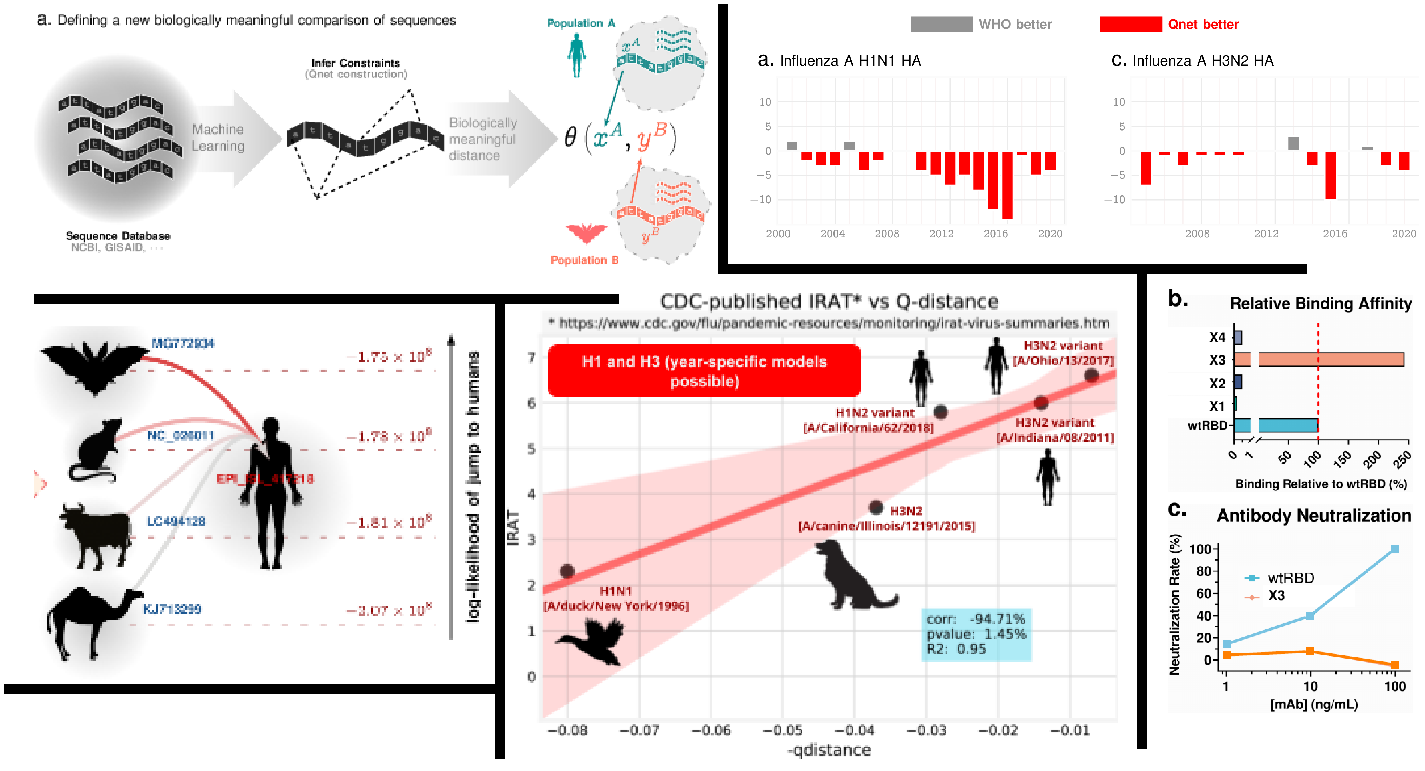
\includegraphics[width=\textwidth]{Figures/fig}
  \captionN{Conceptual framework and current results}\label{fig1}
  \vspace{-10pt}
  
\end{figure}
  \vspace{-10pt}

\paragraph*{Fundraising} To date $\approx$100K has been allocated, including  BIG funding + development funding from Chattopadhyay Lab. We have pending proposals at NSF (PIPP program, 1M USD, summer 2022) and NIH (NIAID R21, 400K, Fall 2022). 

\clearpage

\clearpage
\mbox{}
\clearpage
\mbox{}
\clearpage
\mbox{}
\clearpage
\mbox{}
\clearpage
\mbox{}
\clearpage
\mbox{}
\clearpage
\mbox{}
\clearpage
\mbox{}
\clearpage
\mbox{}
\clearpage
\mbox{}
\clearpage
\mbox{}
\clearpage
\mbox{}
\clearpage
\mbox{}
\clearpage
\mbox{}
\clearpage
\mbox{}
\clearpage
\mbox{}
 
\setcounter{page}{1}

\section*{Knowledgeable Experts in the field}
\DQS{Need 5, please suggest}
1. Peter Hraber\\
Theoretical Biology \& Biophysics Group, T-6\\
Theoretical Division\\
Los Alamos National Laboratory\\
PO Box 1663, MS K710\\
Los Alamos, NM 87545\\
phone: 505 665 7491\\
email: phraber@lanl.gov\\

Dr. Hraber is an expert in  theoretical biology and biophysics,  focusing in  computational immunology, evolution, and statistical genetics, and is well-suited to evaluate the interplay of mathematical modeling, evolutionary dynamics and immunological aspects of the proposed project.
\vskip 1em
\hrule

2. Patrick Wilson\\
Assistant Professor\\
Drukier Institute for Children's Health\\
Weill Cornell Medicine\\
1300 York Avenue\\
New York, NY 10065\\
phone: 212 746 4111\\
email: pcw4001@med.cornell.edu\\

Prof. Wilson is an immunologist with extensive experience in characterization of human immune responses, with definitive work in influenza vaccine designs and B cell biology.
\vskip 1em
\hrule

3. Balaji Manicassamy\\
Associate Professor of Microbiology and Immunology\\
Iowa State University\\
3-430 Bowen Science Building\\
51 Newton Rd\\
Iowa City, IA 52242\\
phone: 319 335 7590\\
email:  balaji-manicassamy@uiowa.edu\\

Prof. Manicassamy is an expert in influenza viruses and respiratory pathogens, with extensive experience in reverse genetics and pathogenesis.
\vskip 1em
\hrule

4.
\vskip 1em
\hrule

5.
\vskip 1em
\hrule
\clearpage

\normalem 

\bibliographystyle{naturemag}
\bibliography{keck,qnet,BibLib1,bioshock_refs,bioshock}

 

\end{document}

